\documentclass[hidelinks,onefignum,onetabnum,final]{siamart220329}  % for arxiv
%\documentclass[review,hidelinks,onefignum,onetabnum,final]{siamart220329}  % for submission

\usepackage{amsfonts,yhmath}
\usepackage{graphicx}
\usepackage{epstopdf}
\ifpdf
  \DeclareGraphicsExtensions{.eps,.pdf,.png,.jpg}
\else
  \DeclareGraphicsExtensions{.eps}
\fi

% Used for creating new theorem and remark environments
\newsiamremark{remark}{Remark}
\newsiamremark{hypothesis}{Hypothesis}
\crefname{hypothesis}{Hypothesis}{Hypotheses}
\newsiamthm{claim}{Claim}
\newsiamthm{conjecture}{Conjecture}
\newsiamremark{example}{Example}

\usepackage{amsopn}
\DeclareMathOperator{\diag}{diag}

\usepackage{bm,bbm,empheq,verbatim,fancyvrb,amssymb}
\usepackage{booktabs,multirow,xspace}
\usepackage{pifont}

\usepackage{tikz}
\usetikzlibrary{decorations.pathreplacing}
\usetikzlibrary{graphs,quotes}

\newcommand{\eps}{\epsilon}
\newcommand{\RR}{\mathbb{R}}

\newcommand{\grad}{\nabla}
\newcommand{\Div}{\nabla\cdot}

\newcommand{\bbf}{\mathbf{f}}
\newcommand{\bg}{\mathbf{g}}
\newcommand{\bn}{\mathbf{n}}
\newcommand{\bu}{\mathbf{u}}
\newcommand{\bv}{\mathbf{v}}
\newcommand{\bw}{\mathbf{w}}
\newcommand{\bx}{\mathbf{x}}
\newcommand{\bz}{\mathbf{z}}

\newcommand{\bX}{\mathbf{X}}

\newcommand{\bzero}{\bm{0}}

\newcommand{\btau}{\bm{\tau}}

\newcommand{\cB}{\mathcal{B}}
\newcommand{\cH}{\mathcal{H}}
\newcommand{\cK}{\mathcal{K}}
\newcommand{\cV}{\mathcal{V}}

\newcommand{\hcK}{\widehat{\cK}}

\newcommand{\nn}{{\text{\textnormal{n}}}}
\newcommand{\pp}{{\text{\textnormal{p}}}}
\newcommand{\qq}{{\text{\textnormal{q}}}}
\newcommand{\rr}{{\text{\textnormal{r}}}}

\newcommand{\ip}[2]{\left<#1,#2\right>}

\newcommand{\XX}{\ding{55}}

\newcommand{\dx}{\, \mathrm{d}x}

\newcommand{\rhoi}{\rho_{\text{i}}}

\DeclareMathOperator*{\argmin}{arg\,min}
\DeclareMathOperator*{\Hull}{Hull}


% running headers and PDF metadata
\headers{Bounds on geometry errors in glacier simulations}{E. Bueler}

\title{Bounds on geometry errors in glacier simulations}

\author{Ed Bueler\thanks{Department of Mathematics and Statistics, University of Alaska Fairbanks, USA (\email{elbueler@alaska.edu}).}}


\begin{document}
\maketitle

\begin{abstract}
The primary data which determine the evolution of glaciation are bedrock elevation and surface mass balance.  From this data the glacier's geometry solves a free-boundary problem over a set of admissible surface elevation functions.  Admissibility requires that the ice surface elevation is above the bedrock topography, equivalently that the ice thickness is nonnegative.  For an implicit time step, the free-boundary problem can be posed in weak form as a variational inequality over a fixed map-plane region, and we conjecture that these continuous-space problems are well-posed in the case of non-shallow Stokes dynamics.  Then we show an abstract estimate for finite element approximations of variational inequality problems over Banach spaces, a theorem in which the nonlinear operator is assumed to be coercive and Lipshitz.  When applied in the glacier case, all terms in the error estimate can be physically-interpreted, and practical approaches to mitigate these errors are proposed.  The resulting computable bounds on the geometry approximation error are demonstrated in an implicit time-stepping glacier simulation based on Stokes dynamics.
\end{abstract}

% REQUIRED
\begin{keywords}
error bounds, finite element methods, glaciers, ice flow, variational inequalities
\end{keywords}

% REQUIRED
%\begin{MSCcodes}
%FIXME
%\end{MSCcodes}


\section{Introduction} \label{sec:intro}

Glacier and ice sheet simulations typically model the ice layer as a free-surface, very-viscous, incompressible, and non-Newtonian fluid \cite{GreveBlatter2009,SchoofHewitt2013}.  For simplicity we will restrict our considerations to simulations of glaciers on land, without floating portions, and we note that an ``ice sheet'' is simply a continent-scale glacier.

Two types of essential input data into such simulations are the bedrock elevation and the surface mass balance (SMB).  We will assume that the bedrock elevation map is constant in time.  By definition, the SMB is the annually-averaged difference of vertically-accumulating snow minus the loss of (liquid) water, through runoff, at the upper surface of the glacier \cite{Cogleyetal2011}, and we assume it depends on time.  Note that elevations are measured here in meters, while the SMB is measured in ice-equivalent units of meters per second.

Thus a glacier simulation takes an initial glacier geometry, the bedrock topography, and the time-dependent climate, i.e.~SMB, as inputs.  It produces the glacier's evolving geometry and flow velocity; these are the output fields of primary scientific value.  The geometry is parameterized by either the (upper) surface elevation or the ice thickness function.  The computed flow velocity is, however, only defined at those three-dimensional locations and times where ice is present, that is, on the evolving 3D domain between the bedrock and ice surface elevations.

Additional complications are common in comprehensive ice sheet models \cite{SchoofHewitt2013}, for example simulation of the internal energy of the ice \cite{Aschwandenetal2012}, and/or of the presence of liquid water within the ice matrix or at the glacier surfaces.  However, here we only consider conservation of mass and momentum, not energy, and furthermore we do not make the shallowness assumptions which are common in comprehensive models.

At a map-plane location and time where a glacier exists the surface elevation exceeds the bedrock elevation, equivalently the ice thickness is positive.  That is, the glacier's geometry must satisfy an inequality to be admissible.  Let $\Omega \subset \RR^2$ be a fixed portion of the earth's surface on which we are interested in glaciation (Figure \ref{fig:stokesdomain}), and let $x\in\Omega$ denote the map-plane coordinate(s).  Assume that we are given, as data, a bed elevation function $b(x)$ and an SMB function $a(t,x)$ for $t\in [0,T]$ and $x\in \Omega$.  (Function spaces for these data will be given below.)  Noting that $a$ is generally signed, in areas where $a>0$ (accumulation; downward arrows in Figure \ref{fig:stokesdomain}) then a glacier will exist, but if $a<0$ (upward arrows) then either a glacier exists with an ablating surface, or no glacier exists.  Determining which situation applies at a given $x\in\Omega$ requires solving a free-boundary problem.

\medskip
\begin{figure}[ht]
\centering
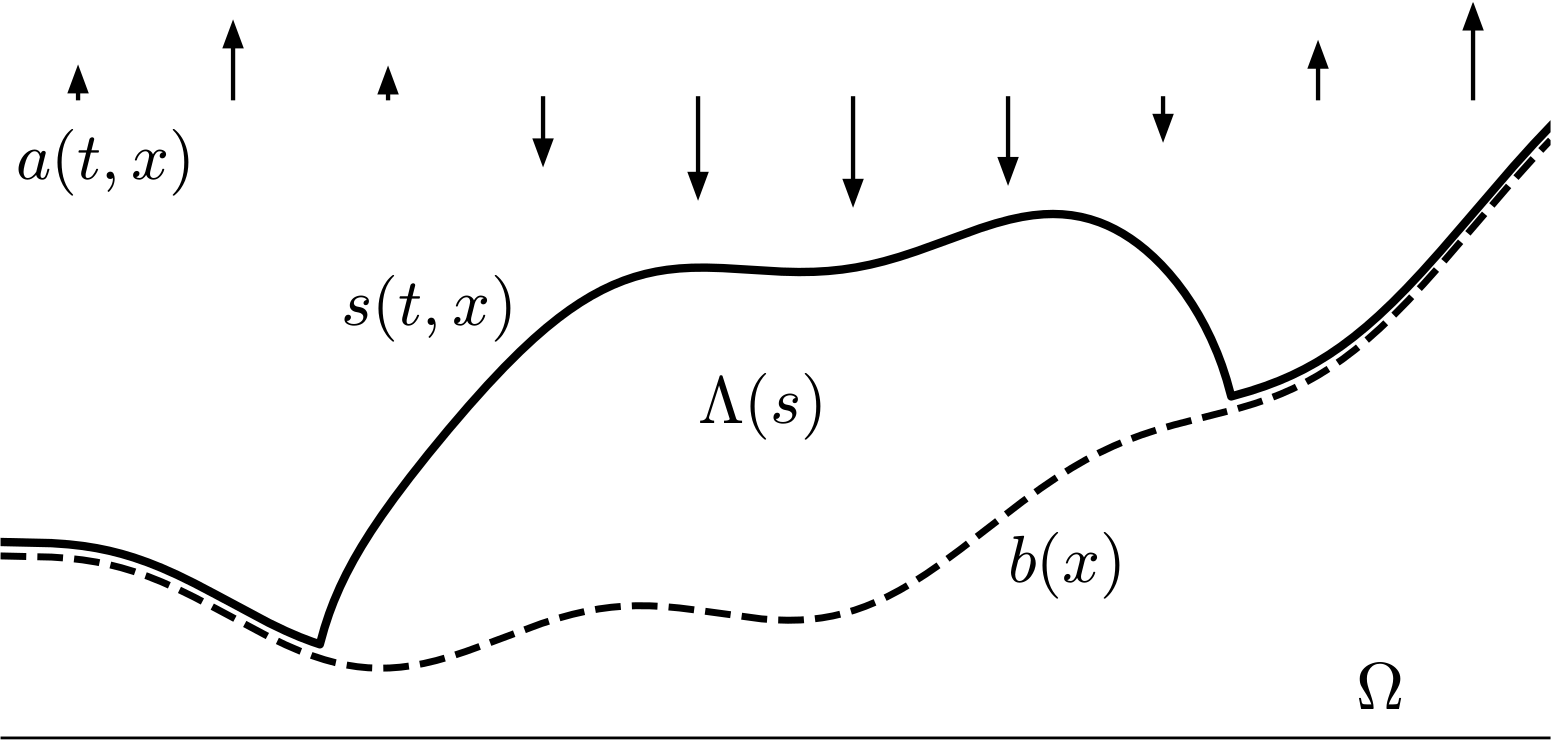
\includegraphics[width=0.65\textwidth]{genfigs/stokesdomain.pdf}
\caption{Glacier notation used in this paper.}
\label{fig:stokesdomain}
\end{figure}

\medskip
Let $s(t,x)$ be the (solution) ice surface elevation.  We will regard this as defined everywhere, but subject to the constraint that the surface $z=s(t,x)$ must be at or above the bedrock, $s(t,x) \ge b(x)$.  Note that some regions in $\Omega$ may have no ice $s(t,x)=b(x)$.  The solution ice velocity $\bu(t,x,z)$ and pressure $p(t,x,z)$ are then defined only on the 3D domain
\begin{equation}
\Lambda(t) = \left\{(x,z)\,:\,b(x) < z < s(t,x)\right\} \subset \Omega \times \RR. \label{eq:icydomain}
\end{equation}
This aspect of glacier modeling deserves emphasis: at any time $t$ the 3D domain $\Lambda(t)$, on which the velocity and pressure are meaningful, is determined by the time-dependent surface elevation $s(t,x)$ which is part of the solution.

Denote the surface value (trace \cite{Evans2010}) of the velocity solution by $\bu|_s$, and let $\bn_s = \left<-\grad s,1\right>$ be a 3D, un-normalized surface normal vector.  For any $T>0$, an infinite-dimensional nonlinear complementarity problem (NCP) \cite{Bueler2021conservation,FacchineiPang2003,SchoofHewitt2013} applies almost everywhere in $[0,T]\times \Omega$:
\begin{subequations}
\label{eq:ncp}
\begin{align}
s - b &\ge 0 \\
\frac{\partial s}{\partial t} - \bu|_s \cdot \bn_s - a &\ge 0 \\
(s - b) \left(\frac{\partial s}{\partial t} - \bu|_s \cdot \bn_s - a\right) &= 0
\end{align}
\end{subequations}
This strong form NCP statement, which will be reformulated as a variational inequality (VI; \cite{KinderlehrerStampacchia1980}) in Section \ref{sec:models} below, assumes that we have extended the surface velocity by zero ($\bu|_s=0$) to the ice-free areas where $s(t,x)=b(x)$.  This NCP says that either a location is ice free ($s-b=0$) and that the climate is locally ablating ($a<0$), or that the surface kinematical equation (SKE) holds:
\begin{equation}
\frac{\partial s}{\partial t} - \bu|_s \cdot \bn_s - a = 0.  \label{eq:ske}
\end{equation}

Well-known equation \eqref{eq:ske} states that the (non-material) surface of the ice moves vertically according to the sum of a component of the ice velocity at the surface and the SMB \cite{SchoofHewitt2013}.  This is a statement of mass conservation at a non-material surface \cite{Aschwandenetal2012}, sometimes wrongly\footnote{Equation \eqref{eq:ske} is not the boundary condition for any identifiable problem.} called a ``kinematical boundary condition'' \cite{GreveBlatter2009}.

The SMB $a(t,x)$ is assumed to be defined everywhere in $\Omega$, regardless of whether a glacier is present or not.  At an ice-free ablative location the value $a(t,x)\le 0$ can be modeled using precipitation and an energy balance \cite{GreveBlatter2009}, for instance by hypothesizing an ice or snow surface, and then computing the balance of snow accumulation versus the total runoff from the available energy for melt.  In other words, the provided SMB at an unglaciated location needs to give the value which a glacier would experience if it were present at that time and place.

Within the ice the simulation needs to conserve mass and momentum.  From \eqref{eq:icydomain} let $\Gamma_s(t) \subset \partial \Lambda(t)$ be the upper surface $z=s$ and
$\Gamma_b(t) \subset \partial \Lambda(t)$ be the base $z=b$.  The models considered here neglect the possibility of fracture-generated cliffs at the ice margin, so we assume $\partial \Lambda(t) = \overline{\Gamma_s(t)} \cup \overline{\Gamma_b(t)}$ at any time.  To conserve mass and momentum within the ice we assume the standard non-shallow ice dynamics model, namely a non-Newtonian and incompressible Stokes problem \cite{GreveBlatter2009,JouvetRappaz2011,SchoofHewitt2013} over $\Lambda(t)$.  To state this model let $D\bu=\frac{1}{2}(\grad \bu + \grad \bu^{\top})$ denote the strain rate tensor.  The shear-thinning ice viscosity, from Glen's power law \cite{GreveBlatter2009}, is given by
\begin{equation}
\nu(D\bu) = \frac{\Gamma}{2} |D\bu|^{\pp-2} \label{eq:glen}
\end{equation}
The exponent $\pp$, often written $\pp=(1/\nn)+1$ in glaciology \cite{GoldsbyKohlstedt2001}, is approximately 4/3.  The coefficient $\Gamma>0$ is determined by the measured properties of ice \cite{GoldsbyKohlstedt2001,GreveBlatter2009}, but we assume it to be constant, modeling an isothermal situation.  Note $\pp=2$ yields a Newtonian fluid with constant viscosity.  If $\rhoi$ is the density of ice and $\bg$ is the acceleration of gravity then,  in this model, a glacier with nonsliding (e.g.~frozen) base \cite{JouvetRappaz2011} has velocity and pressure solving the following equations:
\begin{subequations}
\label{eq:stokes}
\begin{align}
- \nabla \cdot \left(2 \nu(D\bu)\, D\bu\right) + \nabla p &= \rhoi \bg && \text{within $\Lambda(t) \subset \RR^3$} \\
\nabla \cdot \bu &= 0 && \text{within $\Lambda(t) \subset \RR^3$} \label{eq:stokes:incomp} \\
\left(2 \nu(D\bu) D\bu - pI\right) \bn_s &= \bzero && \text{on $\Gamma_s(t)$}\label{eq:stokes:stressfreesurface} \\
\bu  &= \bzero && \text{on $\Gamma_b(t)$}
\end{align}
\end{subequations}
Note that boundary condition \eqref{eq:stokes:stressfreesurface} says that the sub-aerial upper surface is stress free, which should not be confused with \eqref{eq:ske}.

In summary at this point, a glacier simulation is an evolving free-surface flow, subject to a signed climate that can add or remove ice, coupled to a nonlinear Stokes problem within an evolving, 3D icy domain.  A well-posed initial/boundary value problem here will require an initial surface elevation $s(0,x)$ and the data $b(x),a(t,x)$.  The solution variables are $s(t,x)$, $\bu(t,x,z)$, and $p(t,x,z)$, with $s$ defined everywhere over $[0,T]\times \Omega$, but subject to $s \ge b$, and with $\bu,p$ defined on $\Lambda(t)$ for each $t$.

The surface elevation $s$ and surface velocity $\bu|_s(t,x)=\bu(t,x,s(t,x))$ are linked by the kinematical NCP \eqref{eq:ncp} which has the time derivative.  The Stokes sub-model \eqref{eq:glen}--\eqref{eq:stokes} acts as an instantaneous ``algebraic'' constraint on the evolution statement in \eqref{eq:ncp}; it acts instantaneously because the flow is very viscous \cite{Acheson1990}.  The coupled, infinite-dimensional problem \eqref{eq:icydomain}--\eqref{eq:stokes} is therefore both a differential algebraic equation (DAE) system \cite{AscherPetzold1998} and an NCP, and thus glacier modeling is nontrivial.

Glacier simulations are commonly formulated using a finite element (FE) method for the Stokes sub-problem \cite{IsaacStadlerGhattas2015,Jouvetetal2008,Pattynetal2008}, or for a shallow approximation thereof.  However, to the author's knowledge all existing non-shallow (Stokes) evolution models use a explicit time-stepping scheme for the geometry, for example as in \cite{Jouvetetal2008} or \cite{LofgrenAhlkronaHelanow2022}, with the one exception of reference \cite{WirbelJarosch2020}.

Each time step of an implicit time-stepping model based on \eqref{eq:icydomain}--\eqref{eq:stokes} will solve a variational inequality (VI) weak formulation \cite{Evans2010,KinderlehrerStampacchia1980}, but here one must choose whether the glacier geometry is parameterized by surface elevation or thickness.  While essentially equivalent in the (continuum) problem, formulations using these different functions have different character when the bedrock is rough.  Specifically when applying the abstract estimate of Section \ref{sec:abstractestimate}, surface elevation $s$ is preferred because of the flow-caused smoothing effect illustrated in Figure \ref{fig:giscross}.  That is, we observe that for land-based glaciers $s(t,x)$ is smoother in $x$ than the thickness $H(t,x) = s(t,x)-b(x)$ because the latter ``inherits'' the lower regularity of the (typically) eroded and/or faulted bedrock topography.

\begin{figure}
\begin{minipage}[t]{0.85\textwidth}
\vspace{0pt}
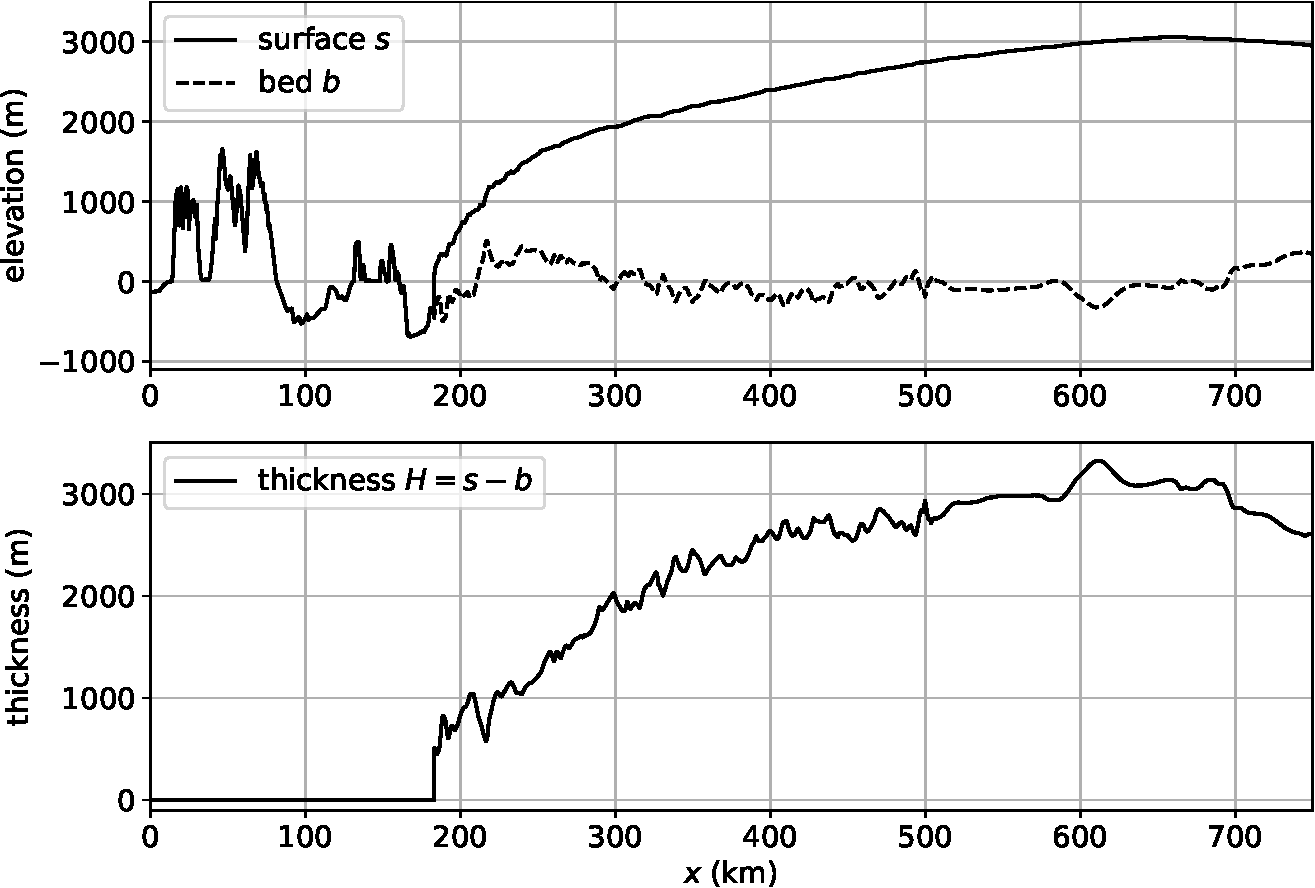
\includegraphics[width=\textwidth]{genfigs/giscross.pdf}
\end{minipage}
\,
\begin{minipage}[t]{0.13\textwidth}
\vspace{10pt}
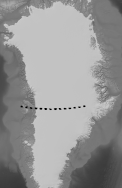
\includegraphics[width=\textwidth]{genfigs/gis/gris-profile-gray.png}
\end{minipage}
\caption{A cross-section of the Greenland ice sheet at $70^\circ$N latitude (inset).  While the ice surface $s$ is relatively smooth because of ice flow (top), the bedrock elevation $b$ is much rougher.  The corresponding ice thickness $H = s-b$ (bottom), though a valid geometry parameterization, inherits the low regularity of $b$.  (Data from \cite{Morlighemetal2017} and A.~Aschwanden, personal communication.)}
\label{fig:giscross}
\end{figure}

FIXME: WHAT WE ACCOMPLISH

This paper is organized as follows.  In Section \ref{sec:models} we reformulate the coupled problem \eqref{eq:icydomain}--\eqref{eq:stokes} as a VI weak form for backward Euler time steps.  Well-posedness for this time-step problem is conjectured over a Banach space of surface elevation functions.  In Section \ref{sec:abstractestimate} we prove an abstract FE error estimate, Theorem \ref{thm:abstractestimate} and its corollaries, for general VI problems involving fully-nonlinear, but coercive and Lipshitz, operators on Banach spaces.  (This estimate extends the classical linear  case by Falk \cite{Falk1974}.)  In Section \ref{sec:application} we apply this theorem to the glacier model time steps.  The distinctive character of non-sliding land-based glaciers, namely how they respond to climate and that they stagnate as they approach zero thickness, implies that certain terms are effectively small, and thus a computable geometry error upper bound follows.  The estimate is demonstrated in Section \ref{sec:demo} on an idealized, but non-trivial, glacier simulation implemented in Firedrake \cite{Hametal2023}.


\section{An implicit time-step model} \label{sec:models}

Let $\{t_n\}$ be an increasing sequence of times, and write $\Delta t = t_n-t_{n-1}$ for any time step.  Suppose $s^n(x)\approx s(t_n,x)$ approximates the unknown surface elevation at time $t_n$.  Using a backward Euler implicit step \cite{AscherPetzold1998}, SKE \eqref{eq:ske} becomes
\begin{equation}
\frac{s^n - s^{n-1}}{\Delta t} - \bu|_{s^n} \cdot \bn_{s^n} - a^n = 0. \label{eq:be:ske}
\end{equation}
Since $a^n$ is the temporal average of $a(t,x)$ over $[t_{n-1},t_n]$, we define the source term
\begin{equation}
\ell^n(x) = s^{n-1}(x) + \int_{t_{n-1}}^{t_n} a(t,x)\,dt, \label{eq:be:source}
\end{equation}
to simply write $\ell^n=s^{n-1}+\Delta t\,a^n$.  Similar to \eqref{eq:ncp}, the implicit step solution $s^n$, now denoted $s$, does not solve \eqref{eq:be:ske} over all of $\Omega$, but rather it solves an NCP:
\begin{subequations}
\label{eq:be:ncp}
\begin{align}
s - b &\ge 0 \label{eq:be:ncp:constraint} \\
s - \Delta t\,\bu|_s \cdot \bn_s - \ell^n &\ge 0 \\
(s - b) \left(s - \Delta t\,\bu|_s \cdot \bn_s - \ell^n\right) &= 0 \label{eq:be:ncp:complementarity}
\end{align}
\end{subequations}
Equation \eqref{eq:be:ncp:complementarity} says that either there is no ice ($s=b$) or that \eqref{eq:be:ske} holds.

The strong form NCP \eqref{eq:be:ncp} has a weak-form variational inequality (VI) version which is suited to both well-posedness theory and finite element (FE) analysis.  However, the precise Banach space $\cV$ of surface elevations in this VI is unknown.  We return to this issue below, but for now the space $\cV$ is abstract.  Admissible surface elevations are from a convex and closed subset of $\cV$:
\begin{equation}
\cK = \left\{r \in\cV\,:\,r \ge b\right\}.  \label{eq:be:admissible}
\end{equation}

We derive the VI form \cite{Bueler2021conservation} as follows, temporarily supposing $s$ is sufficiently-regular to solve NCP \eqref{eq:be:ncp}.  Let $\Omega_I$ be a (measurable) subset of $\Omega$ on which constraint \eqref{eq:be:ncp:constraint} is inactive, so a glacier is present: $\Omega_I \subset \{x\,:\,s(x)>b(x)\}$.  Because \eqref{eq:be:ske} holds on $\Omega_I$ it follows by integration that
\begin{equation}
\int_{\Omega_I} \left(s - \Delta t\,\bu|_s \cdot \bn_s - \ell^n\right)\,(r-s) = 0.  \label{eq:inactivetruth}
\end{equation}
for all $r\in\cK$.  On the other hand, suppose $\Omega_A \subset \{x\,:\,s(x)=b(x)\} \subset \Omega$ is a subset of the active (ice-free) region.  Note that $r-s=r-b\ge 0$ on $\Omega_A$ for $r\in\cK$, and observe that $\ell^n - b \le 0$ on $\Omega_A$ because otherwise, assuming continuity of $b$, $s^{n-1}$, and $a^n$, a glacier would still be present (or would have appeared) somewhere in $\Omega_A$, a contradiction.  Using $\bu|_s=0$ on $\Omega_A$, i.e.~velocity extension by zero, and because $b-\ell^n \ge 0$ and $r-s\ge 0$ on $\Omega_A$, integration now yields an inequality:
\begin{equation}
\int_{\Omega_A} \left(s - \Delta t\,\bu|_s \cdot \bn_s - \ell^n\right)\,(r-s) = \int_A \left(b - \ell^n\right)\,(r-b) \ge 0.  \label{eq:activetruth}
\end{equation}
Almost everywhere $\Omega$ is either covered by glacier (in some $\Omega_I$) or ice free (in $\Omega_A$), thus application of \eqref{eq:inactivetruth} or \eqref{eq:activetruth} justifies the following VI model for $s \in \cK$:
\begin{equation}
\int_\Omega \left(s - \Delta t\,\bu|_s \cdot \bn_s\right)\,(r-s) \ge \int_\Omega \ell^n \,(r-s) \quad \text{for all } r \in \cK. \label{eq:be:viearly}
\end{equation}
This inequality is meaningful in advance of knowing its solution; it does not require knowledge of the ice-covered part of the domain.
	
Next, for $s\in \cV$ we state the weak form of the Stokes equations \eqref{eq:stokes} on the domain $\Lambda(t)$ defined by \eqref{eq:icydomain}, now denoted simply by $\Lambda$.  Note that this Stokes problem computes the field $\bu|_s$ which appears in VI \eqref{eq:be:viearly}.  Here the relevant function spaces are well-known.  Denote by $W^{k,r}(\Lambda)$ the Sobolev space of functions with $k$ weak derivatives which are $r$th-power integrable \cite{Evans2010}.  We will assume that the ice base $\Gamma_b\subset\partial \Lambda$, on which a Dirichlet condition $\bu=\bzero$ holds, has positive measure.  Otherwise we suppose that the boundary $\partial \Lambda$ is stress-free.  Recall that $\pp=(1/\nn)+1\approx 4/3$.  Let $W_b^{1,\pp}(\Lambda)^{3}$ be the space of velocity functions which are zero along $\Gamma_b$.  Define
\begin{equation}
\mathcal{M}_\Lambda = W_b^{1,\pp}(\Lambda)^3 \times L^\qq(\Lambda)  \label{eq:mixed}
\end{equation}
as the (mixed) space of admissible velocity and pressure pairs, where $\qq=\pp/(\pp-1)\approx 4$ is the conjugate exponent.  The Glen-Stokes mixed solution $(\bu,p) \in \mathcal{M}_\Lambda$ satisfies the weak form
\begin{equation}
F_\Lambda(\bu,p)[\bv,q] = \int_\Lambda 2 \nu(|D\bu|) D\bu : D\bv - p \Div\bv - (\Div\bu) q - \rhoi \bg \cdot \bv = 0 \label{eq:glenstokesweak}
\end{equation}
for all $(\bv,q) \in \mathcal{M}_\Lambda$, where the viscosity $\nu(|D\bu|)$ is defined by \eqref{eq:glen}.

Jouvet and Rappaz \cite{JouvetRappaz2011} prove that \eqref{eq:glenstokesweak} is well-posed under the above assumptions if also the Neumann portion of $\partial\Lambda$ is $C^1$; we return to this regularity concern below.  They show well-posedness via the equivalence of \eqref{eq:glenstokesweak} and minimization of a convex and coercive functional over the divergence-free subspace.  Observe that if the solution to \eqref{eq:glenstokesweak} is sufficiently regular then it satisfies strong equations \eqref{eq:stokes}.

The well-posedness of problem \eqref{eq:glenstokesweak} allows us to create a well-defined map from the surface $s=s^n$ to the surface value of the velocity solution $\bu=\bu^n$ .  The map is defined via definition \eqref{eq:icydomain} of $\Lambda=\Lambda(t_n)$, then the solution of \eqref{eq:glenstokesweak} over that domain, and then evaluation of the trace of $\bu$ over $\Gamma_N\subset \partial\Lambda$.  Concretely we define the \emph{surface motion map} $\Phi:\cV \to \cV'$ from the trace of $\bu$ and using the weak derivatives of $s$:
\begin{equation}
\Phi(s) = - \bu|_s\cdot \bn_s \label{eq:be:Phidefine}
\end{equation}
For any surface elevation $s$ so that \eqref{eq:glenstokesweak} is well-posed, this map evaluates the dynamical term in SKE \eqref{eq:be:ske}, and so we can define a final weak form operator $F_{\Delta t}:\cV\to\cV'$:
\begin{equation}
\ip{F_{\Delta t}(s)}{r} = \Delta t\,\ip{\Phi(s)}{r} + \int_\Omega s r = \int_\Omega \left(s - \Delta t\, \bu|_s \cdot \bn_s\right) r.  \label{eq:be:Fdefine}
\end{equation}

Now VI problem \eqref{eq:be:viearly} can be re-written using well-defined operators, as long as $\cV$ has been chosen in an appropriate manner.  Specifically, the solution surface elevation $s$ needs to be regular enough so that the corresponding Stokes problem is well-posed.  Also we assume, reasonably, that the source term $\ell^n$ defined in \eqref{eq:be:source} provides an element of the dual space $\cV'$.  Then we seek $s = s^n \in \cK$ so that
\begin{equation}
\ip{F_{\Delta t}(s)}{r-s} \ge \ip{\ell^n}{r-s} \quad \text{for all } r \in \cK. \label{eq:be:vi}
\end{equation}
This VI form is our preferred weak form associated to the strong-form NCP statement \eqref{eq:be:ncp} of the implicit time step.

VI problem \eqref{eq:be:vi} is the weak form corresponding to NCP \eqref{eq:be:ncp}, and there is general agreement among glaciologists that a backward Euler step for a non-sliding and isothermal glacier would satisfy the conditions of that NCP.  For instance, numerical ice sheet models \cite{IsaacStadlerGhattas2015,WirbelJarosch2020} are based upon this Stokes model, and furthermore the SKE is the standard model for surface geometry evolution \cite{GreveBlatter2009,SchoofHewitt2013}.  However, the bounds on numerical geometry errors proven in Sections \ref{sec:abstractestimate} and \ref{sec:application} below depend on a well-posed problem for the continuum surface elevation.  Because no results known to this author prove well-posedness for \eqref{eq:be:vi} or similar, we conjecture it to be true so as to consider the errors made in the FE approximation.

\begin{conjecture} \label{conj:wellposed:be}
There exists an exponent $\rr$ so that if $\cV = W^{1,\rr}(\Omega)$ then, for all sufficiently-small values $\Delta t>0$, there exists a unique solution to VI problem \eqref{eq:be:vi}.
\end{conjecture}

Certain well-posedness results are known to hold for shallow approximations of problem \eqref{eq:be:vi}.  For the shallow ice approximation (SIA) the ice geometry is often parameterized using the ice thickness, in which case, by incompressibility, the SKE is replaced by a mass continuity or Saint Venant equation \cite{JouvetBueler2012}.  In this case the constraint set is $\tilde{\cK} = \{H\ge 0\}$ where $H=s-b$ is the ice thickness.   For the steady SIA model, with arbitrary smooth bed elevations, existence is known, with a power of $H$ in an identified Sobolev space.\footnote{However, the space of functions whose powers are in a $W^{1,\qq}$ space is not generally even a vector space.  For example, relevant to typical powers used for ice sheets, if $f(x)=(x-1/2)^{3/8} \chi_{[1/2,1]}(x)$ and $g(x)=1$ then $f,g \in \cV = W^{1,4}([0,1])$ but $f+g\notin \cV$.}  That is, there exists $\eta = H^{2\qq/(\qq-1)} \in \subset W^{1,\qq}(\Omega)$ solving the power-transformed VI problem \cite{JouvetBueler2012}; see also \cite{Calvoetal2003,PiersantiTemam2023} regarding the flat-bed and time-dependent case.  On the other hand, the solution regularity from solving the SIA problem likely does not correspond to the regularity of a surface elevation solution of \eqref{eq:be:vi} using non-shallow (Stokes) dynamics.  In fact, it is well-known that the wavelength-dependent surface response of the Stokes model has a quite different small wavelength limit relative to the diffusive SIA model \cite[for example]{Pattynetal2008}.

More generally, it is not very clear what theoretical claims should be made about the shapes of glacier and ice sheet margins, speaking here of the grounded case.  The SIA theory suggests root-type (fractional-power) shapes \cite{Bueleretal2005} with unbounded gradients (Figure \ref{fig:margins}.  On the other hand, earlier glacier modeling often hypothesized a ``wedge'' shape with a finite gradient, and in reality fracture, crevasse, and cliffs features are common at glacier margins.
% CITE FOR wedge?

\begin{figure}
\begin{center}
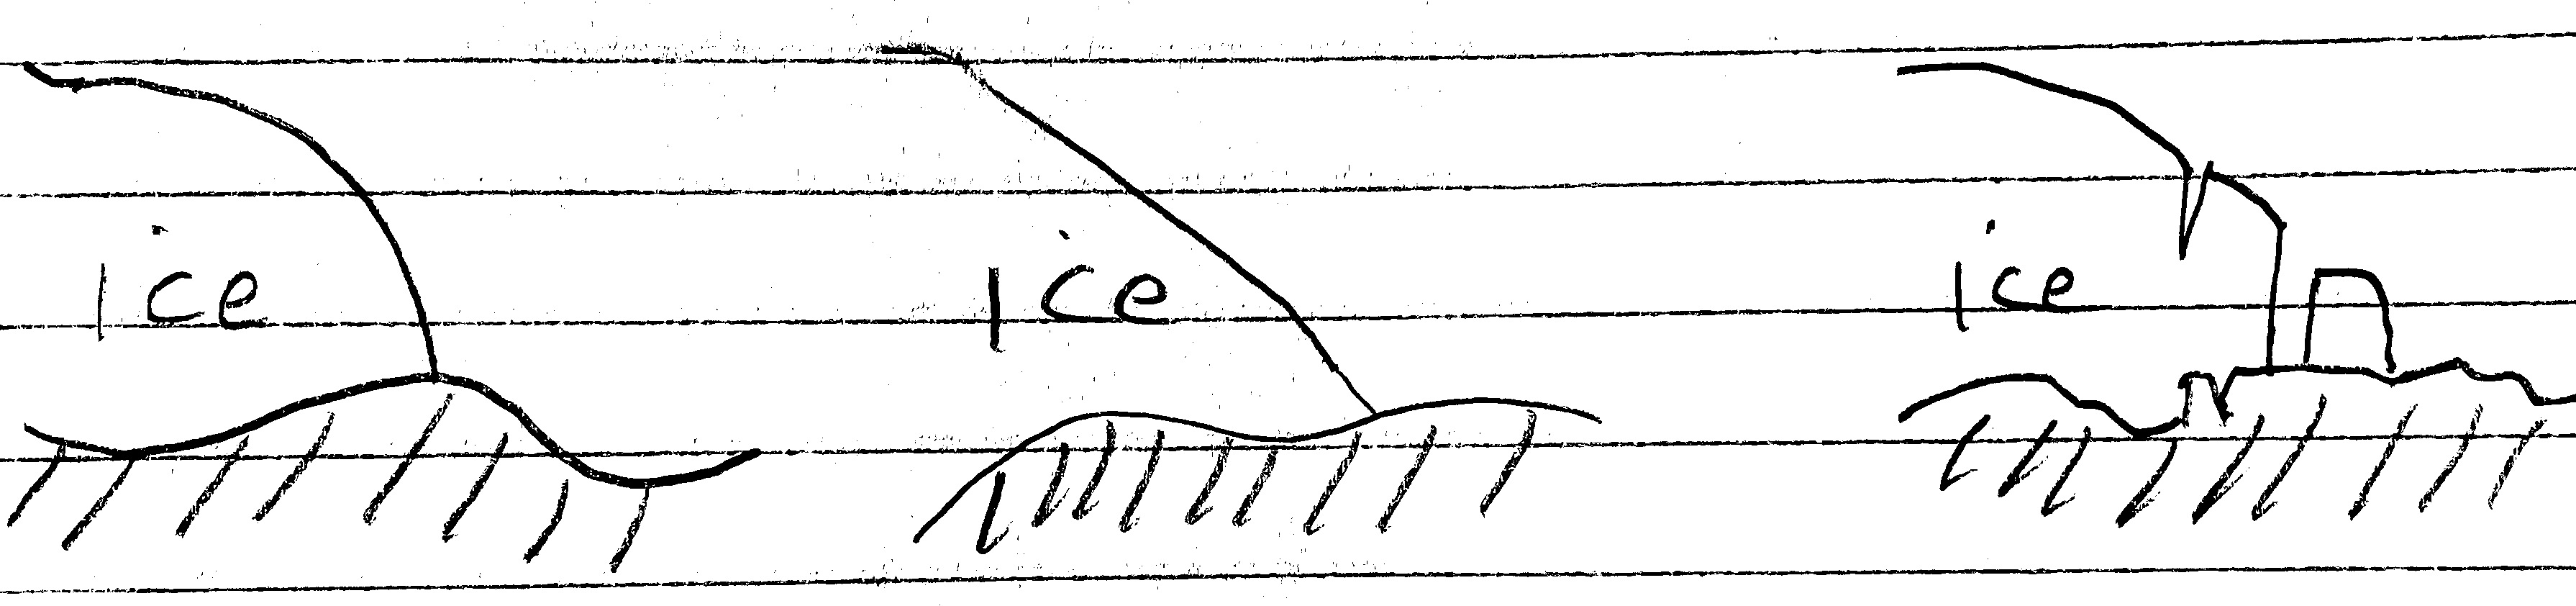
\includegraphics[width=0.8\textwidth]{figs/margins.jpg}
\end{center}
\caption{In which Sobolev space should we seek the surface elevation function?  This question relates to the shape of the ice margin.  The shallow ice theory yields a fractional power shape (left).  Glaciological tradition often hypothesizes a ``wedge'' shape (center).  On the other hand, real glacier margins often have fractures and cliffs.} %FIXME replace with better figure
\label{fig:margins}
\end{figure}

As a mathematical matter, Conjecture \ref{conj:wellposed:be} only addresses the well-posedness of each implicit time-step problem, and this does not suffice to show well-posedness of our original time-dependent problem.  Without making a further formal conjecture, we also suppose that the parabolic VI problem corresponding to time-dependent NCP \eqref{eq:ncp} would also be well-posed.  On the other hand, the results in the next two Sections are only based on Conjecture \ref{conj:wellposed:be}.


\section{Abstract error estimate} \label{sec:abstractestimate}

We now consider an abstract variational inequality (VI) \cite{KinderlehrerStampacchia1980} problem, but we will return to \eqref{eq:be:vi} in section \ref{sec:application}.  Let $\cV$ be a real reflexive Banach space with norm $\|\cdot\|$ and topological dual space $\cV'$.  Denote the dual pairing of $\phi \in \cV'$ and $v\in\cV$ by $\ip{\phi}{v} = \phi(v)$, and define the (Banach space) norm on $\cV'$ by $\|\phi\|_{\cV'} = \sup_{\|v\|=1} |\!\ip{\phi}{v}\!|$.  Let $\cK \subset \cV$ be a nonempty, closed, and convex subset, the constraint set; elements are said to be admissible.  For a continuous, but generally nonlinear, operator $f:\cK \to \cV'$, and a linear source $\ell\in \cV'$, the VI problem is to find $u\in \cK$ such that
\begin{equation}
\ip{f(u)}{v-u} \ge \ip{\ell}{v-u} \quad \text{for all } v\in \cK. \label{eq:vi}
\end{equation}
The best known example of a problem in form \eqref{eq:vi} is the obstacle problem for the Laplacian operator; see \cite{Ciarlet2002,Evans2010,KinderlehrerStampacchia1980} for the theory and FE analysis of that problem.

\begin{definition} \label{def:monotonepcoercive}
An operator $f:\cK \to \cV'$ is said to be \emph{monotone} if
\begin{equation}
\ip{f(v)-f(w)}{v-w} \ge 0 \qquad \text{for all } v,w \in \cK \label{eq:monotone}
\end{equation}
and \emph{strictly monotone} if equality in \eqref{eq:monotone} implies $v=w$.  Let $\pp>1$.  The operator is \emph{$\pp$-coercive \cite{Bueler2021conservation}} if there exists $\alpha>0$ such that
\begin{equation}
\ip{f(v)-f(w)}{v-w} \ge \alpha \|v-w\|^\pp \qquad \text{for all } v,w \in \cK. \label{eq:pcoercive}
\end{equation}
\end{definition}

Clearly, if $f$ is $\pp$-coercive then it is monotone and strictly monotone, in which case any solution of \eqref{eq:vi} is unique.  Furthermore, it is well-known that if $f:\cK \to \cV'$ is also continuous on finite-dimensional subspaces then VI \eqref{eq:vi} has a solution \cite[Corollary III.1.8]{KinderlehrerStampacchia1980}.  Thus $\pp$-coercivity and continuity of $f$ implies well-posedness for \eqref{eq:vi}.
% \cite{Peral1997} uniform continuity over bounded sets for p-Laplacian: Thm A.0.6

\begin{definition} \label{def:lipshitz}
For $\rho>0$ let $B_\rho = \{v\in \cV\,:\,\|v\|\le \rho\}$.  We say $f:\cK \to \cV'$ is \emph{Lipshitz on bounded subsets of $\cK$} if for every $\rho>0$ there is $C(\rho)>0$ so that if $v,w \in B_\rho \cap \cK$ and $z\in\cV$ then $|\ip{f(v)-f(w)}{z}| \le C(\rho) \|v-w\| \|z\|$.
\end{definition}

Equivalently to definition \ref{def:lipshitz}, $f$ is Lipschitz on bounded subsets of $\cK$ if
\begin{equation}
\|f(v)-f(w)\|_{\cV'} \le C(\rho) \|v-w\| \quad \text{ for all } v,w \in B_\rho \cap \cK.  \label{eq:liponbounded}
\end{equation}
Observe that definitions \ref{def:monotonepcoercive} and \ref{def:lipshitz} do not require $f$ to be defined on all of the vector space $\cV$, but rather only on $\cK$.

FIXME finite element space $\cV_h \subset \cV$, constraint set $\cK_h\subset \cV_h$, note generally $\cK_h \nsubseteq \cK$.  let $f_h:\cK_h\to\cV'$.  the FE VI problem approximating \eqref{eq:vi} is
\begin{equation}
\ip{f_h(u_h)}{v_h-u_h} \ge \ip{\ell}{v_h-u_h} \quad \text{for all } v_h\in \cK_h. \label{eq:fe:vi}
\end{equation}
we assume this problem is also well-posed FIXME FLESH OUT AND NOTE $f_h\ne f$ WOULD BE POSSIBLE

FIXME MOVE TO COROLLARY Now assume that $\cV$ continuously and densely embeds in a larger Banach space $\cB$:
\begin{equation}
\cV \hookrightarrow \cB, \quad \overline{\cV} = \cB
\end{equation}
Observe that $\cB' \subset \cV'$ is a subspace.  Our main example will be where $\cV=W^{1,p}(\Omega)$ and $\cB=L^p(\Omega)$, but compare the Hilbert-space case in \cite{Falk1974} and \cite[section 5.1]{Ciarlet2002}.

A key concept in what follows is that $f(u)-\ell$ is generally nonzero when $u$ solves \eqref{eq:vi}.  Instead, a nonlinear complementarity problem holds, at least in sufficiently regular cases, as in \cite[Exercise 5.1.1]{Ciarlet2002}  and \cite[section 7]{BuelerFarrell2024}, for example.  Only for $u$ in the interior of $\cK$ should we expect equality (i.e.~$f(u)=\ell$).

The following abstract error estimate extends \cite{Falk1974} and Theorem 5.1.1 in \cite{Ciarlet2002}, as will be shown in corollaries.  We assume neither that $f$ is linear, nor that $f_h=f$, but we must extend the domain of $f$ to include the finite element solution.

\begin{theorem} \label{thm:abstractestimate}  Suppose $u\in\cK$ solves \eqref{eq:vi} and $u_h\in\cK_h$ solves \eqref{eq:fe:vi}.  Define
\begin{equation}
\hcK = \overline{\Hull{(\cK \cup \cK_h)}}  \label{eq:convexhull}
\end{equation}
as the closure in $\cV$ of the convex hull of $\cK \cup \cK_h$, and suppose that $f$ can be extended to $\hcK$.  For $1<\pp<\infty$ assume $f$ is $\pp$-coercive over $\hcK$ with constant $\alpha>0$, and that it is Lipshitz on bounded sets of $\hcK$.  Let $R_h=\max\{\|u\|,\|u_h\|\}$.  Then there is a constant $c=c(\alpha,R_h)>0$ so that
\begin{align}
\|u-u_h\|^p &\le \quad \frac{2}{\alpha} \inf_{v\in\cK} \ip{f(u)-\ell}{v-u_h} \label{eq:abstractestimate} \\
   &\quad + \frac{2}{\alpha} \inf_{v_h\in\cK_h} \ip{f(u)-\ell}{v_h-u} \notag \\
   &\quad + \frac{2}{\alpha} \ip{f(u_h)-f_h(u_h)}{u_h} \notag \\
   &\quad + \inf_{v_h\in\cK_h} c \|u - v_h\|^\qq \notag
\end{align}
\end{theorem}

\begin{proof}  Consider arbitrary elements $v\in\cK$ and $v_h\in\cK_h$.  Rewrite VIs \eqref{eq:vi} and \eqref{eq:fe:vi}, as follows:
\begin{align*}
\ip{f(u)}{u}     &\le \ip{f(u)}{v} + \ell(u-v),  \\
\ip{f_h(u_h)}{u_h} &\le \ip{f_h(u_h)}{v_h} + \ell(u_h-v_h).
\end{align*}
It follows from $\pp$-coercivity over $\hcK$ and these inequalities that
\begin{align*}
\alpha \|u-u_h\|^\pp &\le \ip{f(u)-f(u_h)}{u-u_h} \\
  &= \ip{f(u)}{u} + \ip{f(u_h)}{u_h} - \ip{f(u)}{u_h} - \ip{f(u_h)}{u} \\
  &= \ip{f(u)}{u} + \ip{f_h(u_h)}{u_h} \\
  &\qquad - \ip{f(u)}{u_h} - \ip{f(u_h)}{u} + \ip{f(u_h)-f_h(u_h)}{u_h} \\
  &\le \ip{f(u)}{v} + \ell(u-v) + \ip{f(u_h)}{v_h} + \ell(u_h-v_h) \\
  &\qquad - \ip{f(u)}{u_h} - \ip{f(u_h)}{u} + \ip{f(u_h)-f_h(u_h)}{u_h} \\
  &= \ip{f(u)}{v-u_h} - \ell(v-u_h) + \ip{f(u_h)}{v_h-u} - \ell(v_h-u) \\
  &\qquad + \ip{f(u_h)-f_h(u_h)}{u_h} \\
  &= \ip{f(u)-\ell}{v-u_h} + \ip{f(u)-\ell}{v_h-u} \\
  &\qquad + \ip{f(u)-f(u_h)}{u-v_h} + \ip{f(u_h)-f_h(u_h)}{u_h}
\end{align*}
Since $u,u_h\in B_{R_h}$, by the Lipshitz assumption over $\hcK$ there is $C(R_h)>0$ so that
\begin{align*}
\alpha \|u-u_h\|^\pp &\le \ip{f(u)-\ell}{v-u_h} + \ip{f(u)-\ell}{v_h-u} \\
  &\qquad + C(R_h) \|u-u_h\|\|u-v_h\| + \ip{f(u_h)-f_h(u_h)}{u_h}
\end{align*}
Now use Young's inequality with $\eps>0$ \cite[Appendix B.2]{Evans2010} on the product of norms:
\begin{align*}
\alpha \|u-u_h\|^\pp &\le \ip{f(u)-\ell}{v-u_h} + \ip{f(u)-\ell}{v_h-u} \\
  &\qquad + C(R_h) \left(\eps\|u-u_h\|^\pp + \tilde C(\eps) \|u-v_h\|^\qq\right) + \ip{f(u_h)-f_h(u_h)}{u_h}
\end{align*}
(Here $\tilde C(\eps) = (\eps \pp)^{-\qq/\pp} \qq^{-1}$.)  Choose $\eps>0$ so that $C(R_h) \eps \le \alpha/2$, and subtract to find
\begin{align*}
\frac{\alpha}{2} \|u-u_h\|^\pp &\le \ip{f(u)-\ell}{v-u_h} + \ip{f(u)-\ell}{v_h-u} \\
  &\qquad + C(R_h) \tilde C(\eps) \|u-v_h\|^\qq + \ip{f(u_h)-f_h(u_h)}{u_h}
\end{align*}
Take infimums to show \eqref{eq:abstractestimate}.
\end{proof}

FIXME MAKE COROLLARY Assume that
\begin{equation}
\|f(u)-\ell\|_{\cB'} < \infty.  \label{eq:fellboundedB}
\end{equation}
Then
\begin{align}
\|u-u_h\|^\pp &\le \inf_{v_h\in\cK_h} c \|u - v_h\|^\qq  \label{eq:NORMabstractestimate} \\
   &\qquad + \inf_{v_h\in\cK_h} \frac{2}{\alpha} \|f(u)-\ell\|_{\cB'} \|u-v_h\|_{\cB} \notag \\
   &\qquad + \inf_{v\in\cK} \frac{2}{\alpha} \|f(u)-\ell\|_{\cB'} \|u_h-v\|_{\cB} \notag
\end{align}

As observed in \cite{Ciarlet2002}, the last quantity in \eqref{eq:abstractestimate}, involving $\|u_h-v\|$ for $v\in\cK$, is generally nonzero in obstacle problems where $\cK_h \nsubseteq \cK$.  This is relevant to glacier models tracking the surface elevation (as opposed to thickness).  In fact, consider obstacle problems where $\cK=\{v(x)\ge \psi(x)\}$, $\psi_h$ is an interpolant of $\psi$, and $\cK_h=\{v_h(x)\ge \psi_h(x)\}$.  Observe that, while $\psi_h(x_j)=\psi(x_j)$ for interpolation nodes $x_j$, generally $\psi_h(x) \ge \psi(x)$ does not hold for all $x\in\Omega$ even if $\psi$ is smooth.  In other words, nodal admissiblity does not imply admissibility.

FIXME draw figure like Ciarlet Figure 5.1.3

On the other hand, the convex hull \eqref{eq:convexhull} is not needed if the nonlinear operator $f=f_h$ is defined on all of $\cV$.  That is, \eqref{eq:abstractestimate} holds if one replaces $\hcK$ with $\cV$ itself.  Furthermore, for \emph{linear} operators defined on the entire vector space, Theorem \ref{thm:abstractestimate} reduces to the abstract error estimate for variational inequalities given in \cite{Falk1974}.  Specifically, suppose $\ip{f(v)}{w}=a(v,w)$ is actually bilinear, $\cV$-elliptic, and continuous on a Hilbert space $\cV$.  Define $A:\cV\to\cV'$, a bounded linear operator, by $Av(w) = a(v,w)$. (Observe that continuity for $a(v,w)$ implies Lipshitz on bounded sets \eqref{eq:liponbounded} for $A$.)  Suppose that $\cV\hookrightarrow \cH$ and $\overline{\cV} = \cH$ for some larger Hilbert space $\cH$, and that $\|Au-\ell\|_{\cH'} < \infty$ so that, up to isomorphism, $Au-\ell \in\cH$.  Then Theorem \ref{thm:abstractestimate} reduces to Theorem 5.1.1 of Ciarlet \cite{Ciarlet2002}, and the result in Falk \cite{Falk1974}.

The following corollary is relevant to glacier models solving for ice thickness (as opposed to surface elevation).  In this case $\cK = \{v\ge 0\}$ consists of all nonnegative functions and $\cK_h=\cK\cap\cV_h$, thus the last term in \eqref{eq:abstractestimate} is zero.

\begin{corollary}  \label{cor:abstractestimate:equalsets}  Suppose $\cK_h \subset \cK$.  Keeping the other assumptions of Theorem \ref{thm:abstractestimate} the same, it follows that
\begin{equation}
\|u-u_h\| \le \left(\inf_{v_h\in\cK_h} \left\{c \|u - v_h\|^\qq + \frac{2}{\alpha} \|f(u)-\ell\|_{\cB'} \|u-v_h\|_{\cB}\right\}\right)^{1/\pp}. \label{eq:abstractestimate:equalsets}
\end{equation}
\end{corollary}

Finally, if $f(u)=\ell$, for example if $u$ is in the interior of $\cK$, then Theorem \ref{thm:abstractestimate} simplifies to, essentially, Cea's lemma \cite{Ciarlet2002}.  The glacier situation here is that the entire domain $\Omega$ is covered in ice, with a positive minimum on the thicknesses.

\begin{corollary}  \label{cor:abstractestimate:interior}
Suppose $f(u)=\ell$.  Keeping the other assumptions of Theorem \ref{thm:abstractestimate} the same, it follows that there is $\tilde c>0$ so that
\begin{equation}
\|u-u_h\| \le \inf_{v_h\in\cK_h} \tilde c \|u - v_h\|^{\qq/\pp} + FIXME. \label{eq:abstractestimate:interior}
\end{equation}
\end{corollary}


\section{Application of the estimate} \label{sec:application}

FIXME apply Theorem \ref{thm:abstractestimate} and talk through what happens

FIXME accomodate the barrier theory from \cite{Bueler2021conservation}


\section{Demonstration of computable geometry error bounds} \label{sec:demo}

FIXME use stuff from multilevel-stokes-geometry


\section{Conclusion} \label{sec:conclusion}

FIXME


\bibliographystyle{siamplain}
\bibliography{estimate}

\end{document}
